\documentclass[11pt]{article}
\usepackage[T1]{fontenc}
\usepackage[utf8]{inputenc}
\usepackage{lmodern,microtype}
\usepackage[margin=1in]{geometry}
\usepackage{amsmath,amssymb,amsthm,mathtools}
\usepackage{booktabs,array,graphicx,xcolor,enumitem}
\usepackage{fancyhdr}
\usepackage[colorlinks=true,linkcolor=blue!45!black,citecolor=blue!45!black,urlcolor=blue!45!black]{hyperref}
\usepackage[nameinlink,noabbrev]{cleveref}
\hypersetup{pdftitle={Nondegenerate symplectic blocks: an exact detector and sharp rank universality},
 pdfauthor={Research prepared for Vladimir Reshetnikov},
 pdfsubject={Exact finite-field probability laws and sharp total-variation asymptotics}}
\definecolor{ink}{HTML}{174E6C}
\pagestyle{fancy}\fancyhf{}
\fancyhead[L]{\small Nondegenerate symplectic blocks}
\fancyhead[R]{\small Research note}
\fancyfoot[C]{\thepage}
\setlength{\headheight}{14pt}
\setlength{\emergencystretch}{2em}
\newtheorem{theorem}{Theorem}[section]
\newtheorem{lemma}[theorem]{Lemma}
\newtheorem{proposition}[theorem]{Proposition}
\newtheorem{corollary}[theorem]{Corollary}
\theoremstyle{definition}\newtheorem{definition}[theorem]{Definition}
\theoremstyle{remark}\newtheorem{remark}[theorem]{Remark}
\newcommand{\F}{\mathbb F}
\newcommand{\E}{\mathbb E}
\newcommand{\Prob}{\mathbb P}
\newcommand{\TV}{d_{\mathrm{TV}}}
\newcommand{\Law}{\mathcal L}
\newcommand{\Mat}{\operatorname{Mat}}
\newcommand{\Sp}{\operatorname{Sp}}
\newcommand{\GL}{\operatorname{GL}}
\newcommand{\nul}{\operatorname{null}}
\newcommand{\rank}{\operatorname{rank}}
\newcommand{\rad}{\operatorname{rad}}
\newcommand{\gb}[2]{\genfrac{[}{]}{0pt}{}{#1}{#2}_{q}}
\newcommand{\ep}[1]{e_{#1}}
\newcommand{\gp}[1]{c_{#1}}
\newcommand{\op}[1]{o_{#1}}
\newcommand{\einf}{e_\infty}
\newcommand{\cinf}{c_\infty}
\newcommand{\oinf}{o_\infty}
\newcommand{\dd}{\mathrm d}
\newcommand{\1}{\mathbf 1}
\DeclareMathOperator{\Alt}{Alt}

\title{\textcolor{ink}{Nondegenerate symplectic blocks:}\\
an exact detector and sharp rank universality}
\author{Research prepared for Vladimir Reshetnikov}
\date{27 November 2026}

\begin{document}
\maketitle
\begin{abstract}
Let $n$ be even and let $A$ be the $n\times n$ block of a uniformly random
symplectic transformation on the perpendicular sum of two nondegenerate
$n$-spaces over $\F_q$. We prove a sharp separation between the information
in the rank of $A$ and the information in its entries. The rank law approaches
that of an independent-entry uniform matrix with total variation
$\frac{c_\infty}{q-1}q^{-n}+O_q(q^{-2n})$, where
$c_\infty=\prod_{j\ge1}(1-q^{-j})$. In contrast, the full matrix laws remain
at a positive distance
$\Delta_q=\prod_{j\ge1}(1-q^{-(2j-1)})(1-\prod_{j\ge1}(1-q^{-2j}))$.
In every finite dimension an exactly optimal test is whether
$J-A^{\mathsf T}JA$ is nonsingular. We derive the complete pointwise
likelihood and prove sharp universality for the nullity of this quadratic
matrix expression under independent-entry sampling.

The result extends the finite-field compression methods in the supplied
GRH development and the ProveIt article into a regime where both observed
spaces grow with the ambient space and neither is Lagrangian. The proof is
unconditional, applies in characteristic two, and is self-contained apart
from elementary finite symplectic geometry, whose needed counts are proved.
Exact rational calculations and independent exhaustive enumeration accompany
the paper. The new mathematical content is the combined optimal-detection
and sharp-universality theorem; the underlying subspace counts have substantial
prior literature. Publication priority is not established, and the new proof
has not been formalized in Lean.
\end{abstract}

\setcounter{tocdepth}{1}\tableofcontents

\section{The result and its meaning}\label{sec:result}

Fix a prime power $q$. All limits keep $q$ fixed. An alternating form has
zero diagonal and satisfies $J^{\mathsf T}=-J$; the zero-diagonal requirement
is retained in characteristic two. Let $n=2m\ge2$ and let $J$ be any
nondegenerate alternating $n\times n$ matrix. We use the symplectic group
for the displayed form:
\[
 \Sp(J\oplus J)=\{g\in\GL_{2n}(\F_q):g^{\mathsf T}
       \begin{pmatrix}J&0\\0&J\end{pmatrix}g
       =\begin{pmatrix}J&0\\0&J\end{pmatrix}\}.
\]
Choose $g$ uniformly and write its first $n$ columns as
\[
 X=\begin{pmatrix}A\\B\end{pmatrix},\qquad A,B\in\Mat_n(\F_q).
\]
Let $U$ denote a uniform element of $\Mat_n(\F_q)$, so its $n^2$ entries
are independent and uniform. The two distributions to be compared are
$P_n=\Law(A)$ and $Q_n=\Law(U)$. Define the \emph{alternating defect}
\begin{equation}\label{eq:defect}
 D(M)=J-M^{\mathsf T}JM.
\end{equation}
It is always alternating, hence has even nullity. Total variation is
$\TV(P,Q)=\frac12\sum_x|P(x)-Q(x)|=\max_E|P(E)-Q(E)|$.

The choice of block matters: each half in this decomposition is
nondegenerate. In the usual ordering with all position coordinates followed
by all momentum coordinates, the first half is instead Lagrangian. Our
block consists of an equal number of complete symplectic coordinate pairs.

Put, with empty products equal to one,
\begin{equation}\label{eq:products}
 c_r=\prod_{i=1}^{r}(1-q^{-i}),\qquad
 e_r=\prod_{i=1}^{r}(1-q^{-2i}),\qquad
 o_r=\prod_{i=1}^{r}(1-q^{-(2i-1)}).
\end{equation}
Their infinite products are positive and satisfy $c_\infty=e_\infty o_\infty$.
Also write
\[
 S_r=|\Sp_{2r}(q)|=q^{2r^2+r}e_r,\quad
 I_{r,d}=\prod_{i=0}^{d-1}(q^{2r-i}-q^i),\quad
 \alpha_n=\frac{e_m^2}{e_{2m}}.
\]
Here $I_{r,d}=0$ for $d>r$, and $\gb ab$ is the Gaussian binomial
coefficient, the number of $b$-subspaces of $\F_q^a$.

\begin{theorem}[Exact optimal detection and sharp separation]\label{thm:main}
For $k\ge0$ define
\begin{equation}\label{eq:F}
 F_q(k)=\frac1{S_k}\sum_{d=0}^{k}\gb{2k}{d} I_{k,d}.
\end{equation}
Then the following statements hold over every finite field.
\begin{enumerate}[label=\textup{(\roman*)},leftmargin=*]
\item For every $M\in\Mat_n(\F_q)$ with $\nul D(M)=2k$,
\begin{equation}\label{eq:likelihood}
 \frac{P_n(M)}{Q_n(M)}=\alpha_n F_q(k).
\end{equation}
This ratio is less than one exactly when $k=0$, and greater than one
exactly when $k\ge1$.
\item The event $\det D(M)\ne0$ is an exactly optimal distinguishing event.
In particular,
\begin{align}
 \TV(P_n,Q_n)&=(1-\alpha_n)\Prob\{D(U)\text{ nonsingular}\}\label{eq:tv1}\\
 &=(\alpha_n^{-1}-1)\Prob\{A\text{ nonsingular}\}.\label{eq:tv2}
\end{align}
\item With $\pi_q(a)=c_\infty q^{-a^2}/c_a^2$ for $a\ge0$, the signed
rank-law difference has the summable expansion
\begin{equation}\label{eq:rankexp}
 \sum_{a\ge0}\left|\Prob(\nul A=a)-\Prob(\nul U=a)
       -q^{-n}\frac{2-q^a}{q-1}\pi_q(a)\right|=O_q(q^{-2n}).
\end{equation}
Consequently
\begin{equation}\label{eq:ranksharp}
 \TV(\Law(\nul A),\Law(\nul U))
   =\frac{c_\infty}{q-1}q^{-n}+O_q(q^{-2n}).
\end{equation}
\item The full matrix laws satisfy
\begin{equation}\label{eq:limit}
 \TV(P_n,Q_n)=\Delta_q+O_q(q^{-n}),\qquad
 \Delta_q=o_\infty(1-e_\infty)=o_\infty-c_\infty>0.
\end{equation}
\end{enumerate}
The constants implied by $O_q$ depend on $q$ only.
\end{theorem}

Thus every test based only on the rank has vanishing advantage, including
an arbitrary decision rule applied to the entire rank value. The determinant
in \eqref{eq:defect} retains a fixed advantage. With equal prior probabilities
for the two models, the best success probability from the entire matrix is
$(1+\TV(P_n,Q_n))/2$, and the rule achieving it is particularly simple:
choose the independent-entry model when $D(M)$ is nonsingular and the
symplectic-block model when it is singular.

For $q=2$,
\[
 \Delta_2=0.13063434670850517643\ldots,
 \qquad \frac{1+\Delta_2}{2}=0.56531717335425258822\ldots.
\]
The rank-only success probability tends to $1/2$. For example, at $n=24$
the exact rank distance is about $1.72131\times10^{-8}$, while the full
distance is about $0.1306343456$. These numbers are exact rational
computations rounded for display, not simulation estimates.

\begin{figure}[t]
 \centering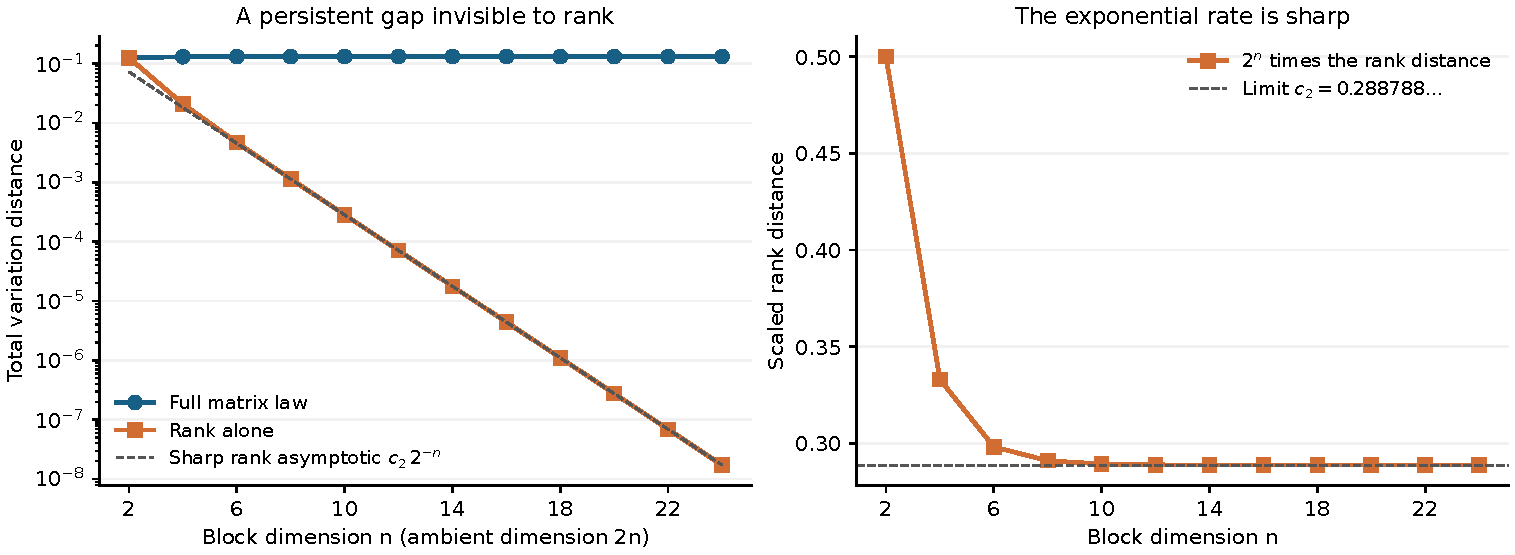
\includegraphics[width=\textwidth]{figures/rank_vs_full.pdf}
 \caption{The binary case, computed from exact finite laws. Left: full
 matrix discrepancy remains positive while rank discrepancy decays.
 Right: the rescaled rank discrepancy converges to the proved sharp
 constant $c_\infty=0.2887880950\ldots$.}
 \label{fig:separation}
\end{figure}

\section{What the supplied repositories contribute}\label{sec:sources}

\subsection{The upstream theorem and the finite mechanism}
We inspected \texttt{lsernau/grh-lean} at commit
\texttt{72fead102f663d5c7a407964a13dc0cf9d977207} \cite{grh}.
Its statement module imports Mathlib directly; its entry module exports
Mathlib's Riemann hypothesis and nonvanishing statements for Dirichlet
$L$-functions to the right of the critical line, with the principal pole
excluded. The precise exported GRH scope is Dirichlet $L$-functions.
The repository reports Lean compilation and independent checker acceptance
using only \texttt{propext}, \texttt{Classical.choice}, and
\texttt{Quot.sound}. We checked statement text and selected proof interfaces;
we did not rerun its complete build or independent kernel replay.

Its main arithmetic argument constructs short integral forms, proves that
translates span nearly all of a target space, and supplies a lower bound
for the corrected Gram determinant of independent integral target forms.
The two determinant estimates cancel a common main term. At the source's
notation-level interface this gives
\[
 m\,\mathrm{totalRemainder}\le f a(\log b)^5.
\]
Parameter selection produces a one-sided square-root-scale prime-remainder
bound. An auxiliary quadratic twist and a Landau argument convert that
bound into zero exclusion. The files
\texttt{New/Reduction/MainInequality.lean} and
\texttt{New/Reduction/Zeros/Criterion.lean} expose these final steps.

The transfer used here begins in
\texttt{New/Spanning/SecondMoment/PositiveType.lean}. For a finite group
representation $\rho:G\to\GL_D(\F_q)$, two $D\times r$ matrices $X_0,X_1$,
and a nonnegative positive-type weight $\Theta$, the source proves a
singular-compression estimate of the form
\begin{equation}\label{eq:upstream}
 q\sum_{\det(X_1^{\mathsf T}\rho(g)X_0)=0}\Theta(g)
 \le 2\sum_g\Theta(g)+q^{r+D/2}Y.
\end{equation}
Here $Y$ bounds the appropriate weighted nonzero-vector stabilizers for
the representation and its contragredient. Positive type realizes
character sums as Gram expressions; finite Fourier orthogonality converts
them into kernel counts. The natural extension is to ask which information
a compression contains beyond its singularity or ordinary rank.
The present theorem answers that question in one critical symplectic
regime. It uses no assumption about zeros of $L$-functions.

\subsection{The increment over the ProveIt collection}
The supplied article was inspected at commit
\texttt{22e5c8b7dda558fd9a50b61465483cb4c0433694} \cite{proveit}.
Its README describes a 621-page consolidation of 103 delivered reports and
760 stated results, and explicitly distinguishes merging from independent
checking. We read the introductory and source material and selected
analytic, local, and matrix sections; this was not a line-by-line audit of
all 621 pages.

The matrix section already includes compression bounds, higher kernel
moments, exact isotropic boundary laws, and a Lagrangian-output example
in which rank tests miss a persistent discrepancy. The later delivered
note \emph{Exact symplectic compression laws} \cite{previous} gives a
general finite-frame law and sharp asymptotics with both frame sizes fixed.
In particular, our finite likelihood can be obtained by specializing that
general law. We give a short direct derivation for transparency.

What is added here is the growing-dimensional nondegenerate/nondegenerate
regime, its complete likelihood sign classification, an exactly optimal
determinant test, its limiting advantage, and the sharp first-order
asymptotics of the rank-law difference. The supplementary quadratic-defect
universality theorem also has a sharp first-order expansion. The ordinary
kernel-isotropy obstruction in a Lagrangian output space is replaced by a
different invariant, $J-M^{\mathsf T}JM$.

\subsection{Classical antecedents and the novelty boundary}
Finite symplectic bases, Gaussian coefficients, and orbit classification by
the induced form are classical. Fulman and Goldstein \cite{FG} establish
sharp convergence results for classical finite-field matrix rank laws.
Pott, Schmidt, and Zhou \cite{PSZ} give exact rank-intersection counts for
two alternating matrices and their sum. Glasby, Niemeyer, and Praeger
\cite{GNP} study direct sums of nondegenerate spaces; De Boeck and Van de
Voorde \cite{DBV} provide exact subspace counts that include antecedents
for the single probability $\Prob(A\text{ nonsingular})$ here.

We do not claim those counts or the classical limiting rank distributions
as new. The contribution is the combined statistical theorem and its direct
quantitative proof. Targeted primary-literature searches did not locate
this exact combination of an optimal defect test, a positive full-matrix
limit, and sharp vanishing rank advantage. That comparison supports a
specific extension claim; it does not certify worldwide priority.

\section{Finite geometry and exact moment identities}\label{sec:counts}

\subsection{Prescribed-form frames}
Let $D$ be even. For a $j$-dimensional alternating space of rank $2s$, write
$t=j-2s$ for its radical dimension. Define $E(D,j,s)$ as the number of
isometric injections of this specified space into a nondegenerate
$D$-dimensional alternating space. It is zero unless
$0\le2s\le j$ and $j-s\le D/2$.

\begin{lemma}[Frame count]\label{lem:frames}
In the feasible range,
\begin{align}
 E(D,j,s)&=\frac{S_{D/2}}{S_{D/2-s}} I_{D/2-s,j-2s}\label{eq:Ecount}\\
 &=q^{Dj-j(j-1)/2}\Phi(D,j,s),\label{eq:Ephi}\\
 \Phi(D,j,s)&=\prod_{i=D/2-j+s+1}^{D/2}(1-q^{-2i}).\label{eq:Phi}
\end{align}
The symplectic group is transitive on these injections. The number of
$j$-subspaces of restricted rank $2s$ in a nondegenerate $D$-space is
\begin{equation}\label{eq:C}
 C(D,j,s)=\frac{E(D,j,s)}{S_s\,|\GL_{j-2s}(q)|\,q^{2s(j-2s)}}.
\end{equation}
\end{lemma}

\begin{proof}
Split the domain into a nondegenerate $2s$-space and its radical. Embedding
the first part gives $S_{D/2}/S_{D/2-s}$ choices, because a symplectic
basis extends and the pointwise stabilizer acts on its perpendicular
complement. In that complement the radical must be an independent
isotropic $t$-frame. After $i$ vectors have been chosen, their perpendicular
space has $q^{D-2s-i}$ elements and their span has $q^i$ elements. The next
vector therefore has $q^{D-2s-i}-q^i$ choices. This proves
\eqref{eq:Ecount}. Extracting powers of $q$ gives \eqref{eq:Ephi}--\eqref{eq:Phi}.
The same basis-completion procedure sends any prescribed frame to any
other and proves transitivity, including for a degenerate domain.

An isometry of the domain preserves its radical. In the displayed split
its blocks are $\left(\begin{smallmatrix}P&0\\R&T\end{smallmatrix}\right)$,
where $P\in\Sp_{2s}(q)$, $T\in\GL_t(q)$, and $R$ is arbitrary.
There are $S_s|\GL_t(q)|q^{2st}$ such isometries. Dividing the injection
count by this number gives \eqref{eq:C}.
\end{proof}

For later use put $\Phi=0$ in the infeasible range. For feasible types,
$e_\infty\le\Phi\le1$. The elementary inequality
$1-\prod_i(1-u_i)\le\sum_i u_i$ gives
\begin{equation}\label{eq:phibound}
 1-\Phi(n,j,s)\le\frac{q^{-n+2j}}{q^2-1},\qquad
 1-\Phi(2n,j,s)\le\frac{q^{-2n+2j}}{q^2-1}.
\end{equation}
These bounds are valid for all $0\le j\le n$ and $0\le2s\le j$;
an infeasible first embedding forces $j>n/2$, when the first right side
is at least one. The second embedding is always feasible.

\subsection{Kernel moments of the block}
Let $Z=\nul A$ and $Z_0=\nul U$. Counting $j$-subspaces in the kernels gives
\begin{equation}\label{eq:blockmoments}
 \mu_j:=\E\gb Zj
  =\sum_s C(n,j,s)\frac{E(n,j,s)}{E(2n,j,s)},\qquad
 \mu_j^0:=\E\gb{Z_0}{j}=\gb nj q^{-nj}.
\end{equation}
Indeed, a specified source $j$-space of restricted rank $2s$ is sent
uniformly to one of $E(2n,j,s)$ frames. Its top block vanishes precisely
when its image lies in the bottom $n$-space, which allows $E(n,j,s)$ choices.
For an independent-entry matrix, annihilating that $j$-space imposes $nj$
independent scalar conditions.

Using $\gb nj q^{-nj}\le c_\infty^{-1}q^{-j^2}$, equations
\eqref{eq:Ephi} and \eqref{eq:phibound} imply the uniform estimate
\begin{equation}\label{eq:muerror}
 |\mu_j-\mu_j^0|
 \le \frac{2}{c_\infty e_\infty(q^2-1)}
       q^{-n-j^2+2j}\qquad(0\le j\le n).
\end{equation}
All sums over $s$ below mean $0\le2s\le j$, with impossible embeddings zero.

\subsection{Kernel moments of the quadratic defect}
Let $R=\nul D(U)$ and let $T$ be the nullity of a uniformly random
alternating $n\times n$ matrix. Both are even.

\begin{lemma}[Defect moments]\label{lem:defectmom}
For $0\le j\le n$,
\begin{align}
 \nu_j:=\E\gb Rj
 &=q^{-2nj+j^2}\sum_s C(n,j,s)E(n,j,s),\label{eq:defectmom}\\
 \nu_j^0:=\E\gb Tj
 &=\gb nj q^{-nj+j(j+1)/2},\label{eq:altmom}\\
 |\nu_j-\nu_j^0|
 &\le\frac{q^{-n-j(j-1)/2+2j}}{c_\infty(q^2-1)}.\label{eq:nuerror}
\end{align}
\end{lemma}

\begin{proof}
Fix a $j$-space $K$ of restricted rank $2s$. If $K\subseteq\ker D(U)$
and $Ux=0$ for $x\in K$, then $J(x,y)=J(Ux,Uy)=0$ for every $y$, so
$x=0$. Thus $U|_K$ is an isometric injection, with $E(n,j,s)$ choices.
After its images have been chosen, each of the remaining $n-j$ basis
vectors has $j$ independent pairing constraints and hence $q^{n-j}$
possible images. Dividing by $q^{n^2}$ gives
$E(n,j,s)q^{-2nj+j^2}$, proving \eqref{eq:defectmom}.

For a uniform alternating matrix, killing a specified $j$-space imposes
$nj-j(j+1)/2$ independent coordinates. This proves \eqref{eq:altmom}.
Substituting \eqref{eq:Ephi} and using \eqref{eq:phibound} gives
\eqref{eq:nuerror}.
\end{proof}

\section{The exact likelihood and the optimal test}\label{sec:likelihood}

The frame $X=(A;B)$ satisfies
\begin{equation}\label{eq:gram}
 A^{\mathsf T}JA+B^{\mathsf T}JB=J.
\end{equation}
Conversely every solution is injective, since the right side is
nondegenerate. Symplectic basis extension shows that these frames are
uniform and number $S_{2m}/S_m$.

Fix $A=M$ and let $\nul D(M)=2k$. Split the domain of $D(M)$ into its
nondegenerate part, of dimension $2m-2k$, and its radical. An image for
the first part under $B$ can be chosen in $S_m/S_k$ ways. The radical
maps into the remaining symplectic $2k$-space with isotropic image. If
this map has rank $d$, its kernel has codimension $d$ and can be chosen
in $\gb{2k}{d}$ ways. For each kernel, its quotient has $I_{k,d}$
isometric injections into that complement. Therefore
\[
 \#\{B:B^{\mathsf T}JB=D(M)\}
  =\frac{S_m}{S_k}\sum_{d=0}^k\gb{2k}{d}I_{k,d}.
\]
Divide by $S_{2m}/S_m$ and by $Q_n(M)=q^{-4m^2}$ to obtain
\eqref{eq:likelihood}.

To determine its sign, first observe
\[
 F_q(0)=1,\qquad F_q(1)=1+\frac q{q^2-1},\qquad
 e_\infty\le\alpha_n<1.
\]
The strict upper bound follows by comparing the first $m$ even-product
factors with the next $m$. For $k\ge2$, retain only the $d=k$ term:
\begin{equation}\label{eq:Fbound}
 F_q(k)\ge q^{-k(k+1)/2}\gb{2k}{k}
       \ge q^{k(k-1)/2}\ge q.
\end{equation}
Here $I_{k,k}/S_k=q^{-k(k+1)/2}$ by direct cancellation. Also
\[
 e_\infty\ge 1-\sum_{i\ge1}q^{-2i}
   =\frac{q^2-2}{q^2-1}>\frac12.
\]
It follows that $\alpha_nF_q(k)>1$ for $k\ge2$. For $k=1$ the same
product bound gives
\[
 e_\infty F_q(1)\ge
 \frac{(q^2-2)(q^2+q-1)}{(q^2-1)^2}>1,
\]
because the numerator minus the denominator is
$q^3-q^2-2q+1>0$ for every integer $q\ge2$.

This proves that all negative mass differences $P_n(M)-Q_n(M)$ occur
exactly at nonsingular defects. Summing those differences proves the
optimality claim and \eqref{eq:tv1}. Finally \eqref{eq:gram} says
$D(A)=B^{\mathsf T}JB$, which is nonsingular exactly when $B$ is invertible.
The half-swap map preserves $J\oplus J$, so $A$ and $B$ have the same
distribution. Hence
\[
 \alpha_n\Prob\{D(U)\text{ nonsingular}\}
   =\Prob\{D(A)\text{ nonsingular}\}
   =\Prob\{A\text{ nonsingular}\},
\]
which proves \eqref{eq:tv2}.

\section{Quantitative inversion of kernel moments}\label{sec:inversion}

Convergence of a few moments does not by itself give total variation, and
unbounded moment problems can be indeterminate. Here finite interpolation
provides an explicit, summable estimate.

For an integer $z\ge0$, counting maps $\F_q^i\to\F_q^z$ by their image gives
\begin{equation}\label{eq:convert}
 q^{iz}=\sum_{j=0}^{i}\left(\prod_{h=0}^{j-1}(q^i-q^h)\right)\gb zj.
\end{equation}
For $0\le a\le n$ define the polynomial
\[
 L_{a,n}(x)=\prod_{\substack{0\le j\le n\\j\ne a}}
                 \frac{x-q^j}{q^a-q^j}.
\]
On possible values of $q^Z$, it equals $\1_{Z=a}$.

\begin{lemma}[Interpolation coefficients]\label{lem:coeff}
For every coefficient index $i$,
\begin{equation}\label{eq:coeff}
 |[x^i]L_{a,n}(x)|
 \le c_\infty^{-3}q^{-a(a+1)/2}q^{-i(i-1)/2}.
\end{equation}
On the even grid $1,q^2,\ldots,q^{2m}$, the corresponding indicator
$L^{\mathrm{ev}}_{a,m}$ for nullity $2a$ satisfies
\begin{equation}\label{eq:evcoeff}
 |[x^i]L^{\mathrm{ev}}_{a,m}(x)|
 \le e_\infty^{-3}q^{-a(a+1)}q^{-i(i-1)}.
\end{equation}
\end{lemma}

\begin{proof}
The constant prefactor in $L_{a,n}$, after writing its factors as
$1-xq^{-j}$, has absolute value
$q^{-a(a+1)/2}/(c_a c_{n-a})$. The sum of products of any $i$ distinct
members of $1,q^{-1},q^{-2},\ldots$ is
\[
 \sum_{0\le r_1<\cdots<r_i}q^{-r_1-\cdots-r_i}
    =\frac{q^{-i(i-1)/2}}{c_i}.
\]
This identity follows by removing the staircase $0,1,\ldots,i-1$ and
summing successive nonnegative gaps. It bounds the absolute coefficient
after any one index is omitted. This proves \eqref{eq:coeff}. Replacing
$q$ by $q^2$ proves \eqref{eq:evcoeff}.
\end{proof}

Combining \eqref{eq:convert} with \eqref{eq:muerror} gives
\begin{equation}\label{eq:powererror}
 |\E q^{iZ}-\E q^{iZ_0}|
 \le C_q q^{-n}\sum_{j=0}^{i}q^{-j^2+(i+2)j}
 \le C'_q q^{-n+(i+2)^2/4}.
\end{equation}
The last bound follows by completing the square and bounding the shifted
Gaussian sum by $\sum_{r\in\mathbb Z}q^{-r^2/4}$.
Apply \cref{lem:coeff} to this estimate. The remaining coefficient sum is
bounded independently of $a,n$ because
\[
 \sum_{i\ge0}q^{-i(i-1)/2+(i+2)^2/4}
 =\sum_{i\ge0}q^{-i^2/4+3i/2+1}<\infty.
\]
Thus
\begin{equation}\label{eq:rankmassbound}
 |\Prob(Z=a)-\Prob(Z_0=a)|
       \le C''_q q^{-n-a(a+1)/2}.
\end{equation}
Summing over $a$ proves the exponential rank-universality bound.

The same argument using \eqref{eq:nuerror} gives
\[
 |\E q^{iR}-\E q^{iT}|\le C_q q^{-n+i(i+5)/2}.
\]
Indeed the exponents $ij-j(j-1)/2+2j$ increase by at least $3$ as $j$
increases to $i$, so their sum is bounded by a constant times its final
term. Multiplying by the even-grid bound leaves the summable series
$\sum_{i\ge0}q^{-i^2/2+7i/2}$. We obtain
\begin{equation}\label{eq:defectmassbound}
 |\Prob(R=2a)-\Prob(T=2a)|\le C_q q^{-n-a(a+1)},
 \qquad \TV(\Law(R),\Law(T))=O_q(q^{-n}).
\end{equation}

\section{Sharp first-order laws}\label{sec:sharp}

This section refines the preceding bounds and proves
\eqref{eq:rankexp}--\eqref{eq:ranksharp}. It also identifies the sharp
constant for defect-nullity universality.

\subsection{A common expansion for the two moment problems}
Let $H$ be a uniform alternating $j\times j$ matrix and put
$2s=\rank H$. Define
\[
 u_j=\frac{q^{-j^2}}{c_j},\qquad
 v_j=\frac{q^{-j(j-1)/2}}{c_j},\qquad \tau=q^{-n},\qquad
 W(H)=\frac{q^{2(j-s)}-1}{q^2-1}.
\]
The probability of a given rank type of $H$ is
\[
 \frac{|\GL_j(q)|}
 {q^{j(j-1)/2}S_s|\GL_{j-2s}(q)|q^{2s(j-2s)}}.
\]
Substituting this and \cref{lem:frames} into the exact moments gives
\begin{align}
 \mu_j&=u_j\E_H\frac{\Phi(n,j,s)^2}{\Phi(2n,j,s)},&
 \mu_j^0&=u_j\E_H\Phi(n,j,s),\label{eq:unifiedrank}\\
 \nu_j&=v_j\E_H\Phi(n,j,s)^2,&
 \nu_j^0&=v_j\E_H\Phi(n,j,s).\label{eq:unifieddefect}
\end{align}

Uniformly for $j\le n$ and all types,
\begin{equation}\label{eq:Phitaylor}
 \Phi(n,j,s)=1-\tau W(H)+O_q(\tau^2q^{4j}),\qquad
 \Phi(2n,j,s)=1+O_q(\tau^2q^{2j}).
\end{equation}
In the feasible range the sum of the omitted factors is precisely
$\tau W(H)$, and the error after the linear term is bounded by its square.
In the infeasible range $\Phi(n,j,s)=0$ and $\tau W(H)\ge1$;
$|1-\tau W(H)|\le\tau^2W(H)^2$ proves the same estimate. The denominator
in \eqref{eq:unifiedrank} is always at least $e_\infty$, so division is
uniformly harmless. It follows that
\begin{align}
 \mu_j-\mu_j^0
 &=-\tau u_j\E_HW(H)+O_q(\tau^2u_jq^{4j}),\label{eq:rankfirstmoment}\\
 \nu_j-\nu_j^0
 &=-\tau v_j\E_HW(H)+O_q(\tau^2v_jq^{4j}).\label{eq:defectfirstmoment}
\end{align}
For $j\ge1$, each fixed nonzero vector is killed by $H$ with probability
$q^{-(j-1)}$. Therefore
\[
 \E_Hq^{\nul H}=1+(q^j-1)q^{-(j-1)},\qquad
 \E_HW(H)=\frac{q^j-1}{q-1}.
\]
The latter identity also holds for $j=0$.

\subsection{Identifying the signed measures}
The limiting square-matrix nullity law and even alternating nullity law are
\begin{equation}\label{eq:classical}
 \pi_q(a)=\frac{c_\infty q^{-a^2}}{c_a^2},\qquad
 \eta_q(2a)=\frac{o_\infty q^{-a(2a-1)}}{c_{2a}},\qquad
 \eta_q(2a+1)=0.
\end{equation}
These classical formulas can be obtained directly: count matrices of a
fixed rank, or choose the radical of an alternating form and a nondegenerate
form on its quotient, and pass to the limit. Their Gaussian moments are
$u_j$ and $v_j$, respectively. The tails of the displayed formulas justify
termwise moment limits. Their masses sum to one, since the same moment
bounds give tightness of the finite distributions.

Define the signed sequences
\begin{equation}\label{eq:signed}
 \delta_q(a)=\frac{2-q^a}{q-1}\pi_q(a),\qquad
 \epsilon_q(2a)=\frac{q+1-q^{2a}}{q^2-1}\eta_q(2a),\quad
 \epsilon_q(2a+1)=0.
\end{equation}
The Gaussian identity
\begin{equation}\label{eq:gaussrec}
 (q^a-q^j)\gb aj=q^j(q^{j+1}-1)\gb a{j+1}
\end{equation}
and the ratios
\[
 (q^{j+1}-1)u_{j+1}=q^{-j}u_j,\qquad
 (q^{j+1}-1)v_{j+1}=qv_j
\]
show that their Gaussian moments are
\begin{equation}\label{eq:signedmoments}
 \sum_a\gb aj\delta_q(a)=-u_j\frac{q^j-1}{q-1},\qquad
 \sum_a\gb aj\epsilon_q(a)=-v_j\frac{q^j-1}{q-1}.
\end{equation}
For example the tilted probability law $(q^a-1)\pi_q(a)$ has moments
$q^ju_j$, while $q^a\eta_q(a)/(q+1)$ has moments $q^jv_j$.

\subsection{Summable remainder after inversion}
Subtract $\tau$ times the first signed measure from the rank-law
difference. By \eqref{eq:rankfirstmoment}, \eqref{eq:signedmoments}, and
\eqref{eq:convert}, its $i$th power moment has absolute value at most
\[
 C_q\tau^2\sum_{j\le i}q^{-j^2+(i+4)j}
   \le C'_q\tau^2q^{(i+4)^2/4}.
\]
Multiplication by \eqref{eq:coeff} leaves a convergent series with exponent
$-i^2/4+5i/2+4$. Thus the error at $a\le n$ is bounded by a constant times
$\tau^2q^{-a(a+1)/2}$, apart from the tail of the infinite signed measure
outside the interpolation grid. That tail is harmless: for $b>n$,
\[
 |L_{a,n}(q^b)|\le
 c_\infty^{-2}q^{nb-n(n+1)/2-a(a-1)/2},\qquad
 |\delta_q(b)|\le C_q q^{-b^2+b}.
\]
The sum over $b>n$, then over $a\le n$, is
$O_q(q^{-n(n+1)/2})$. Multiplication by $\tau$ makes it
$O_q(\tau^2)$; the omitted masses themselves are smaller. This proves
\eqref{eq:rankexp}.

For the defect, the analogous power-moment remainder is at most
$C_q\tau^2q^{i(i+9)/2}$. Multiplying by \eqref{eq:evcoeff} leaves the
convergent series with exponent $-i^2/2+11i/2$. At even $b>2m=n$ the
infinite signed tail is bounded using
\[
 |L^{\mathrm{ev}}_{a,m}(q^b)|\le
 e_\infty^{-2}q^{mb-m(m+1)-a(a-1)},\qquad
 |\epsilon_q(b)|\le C_q q^{-b(b-3)/2}.
\]
Its contribution after multiplication by $\tau$ is
$O_q(q^{-n-n^2/4+1})$, hence $O_q(q^{-2n})$ for all large even $n$;
the finitely many smaller $n$ are absorbed in the constant. We have proved
the following companion theorem.

\begin{theorem}[Sharp quadratic-defect universality]\label{thm:defect}
Let $U$ and $T$ be as in \cref{lem:defectmom}. Then
\begin{equation}\label{eq:defectexp}
 \sum_{a\ge0}\left|\Prob(\nul D(U)=a)-\Prob(T=a)
              -q^{-n}\epsilon_q(a)\right|=O_q(q^{-2n}),
\end{equation}
and consequently
\begin{equation}\label{eq:defectsharp}
 \TV(\Law(\nul D(U)),\Law(T))
  =\frac{q\,o_\infty}{q^2-1}q^{-n}+O_q(q^{-2n}).
\end{equation}
\end{theorem}

For the rank signed measure $\delta_q$, the only positive mass is at
$a=0$; at $q=2,a=1$ it is zero. Its positive mass totals
$c_\infty/(q-1)$, proving \eqref{eq:ranksharp}. For the defect signed
measure, the only positive mass is at $a=0$, of size
$q o_\infty/(q^2-1)$, proving \eqref{eq:defectsharp}.

Finally $\Prob(\nul U=0)=c_n=c_\infty+O_q(q^{-n})$ and
$\alpha_n=e_\infty+O_q(q^{-n})$. Equation \eqref{eq:tv2} gives
\eqref{eq:limit}, completing \cref{thm:main}.

\begin{corollary}[First correction to the full-matrix distance]
The positive limiting discrepancy has the refinement
\[
 \TV(P_n,Q_n)=\Delta_q+
 \frac{2o_\infty}{q^2-1}\bigl(q-(q+1)e_\infty\bigr)q^{-n}
       +O_q(q^{-2n}).
\]
The coefficient of $q^{-n}$ is strictly negative.
\end{corollary}
\begin{proof}
The product tails and \eqref{eq:rankexp} give
\[
 \alpha_n=e_\infty\left(1+\frac{2q^{-n}}{q^2-1}+O_q(q^{-2n})\right),
 \quad
 \Prob(Z=0)=c_\infty\left(1+\frac{2q^{-n}}{q-1}+O_q(q^{-2n})\right).
\]
Insert these in \eqref{eq:tv2}. For $q>2$, the product lower bound gives
$e_\infty\ge(q^2-2)/(q^2-1)>q/(q+1)$. For $q=2$ the product inequality
is strict, so $e_\infty>2/3$ as well.
\end{proof}

\begin{remark}
The defect \emph{nullity} is asymptotically classical. The full Gram matrix
$U^{\mathsf T}JU$ is not asymptotically uniform among alternating matrices.
For example its likelihood with respect to uniform alternating sampling
at corank $2k$ is $e_mF_q(k)$, which has a persistent dependence on $k$.
Translating that matrix by $J$ cannot eliminate its full-distribution bias.
The proof above counts kernels of the translated defect directly; it does
not assume a false full-matrix equidistribution statement.
\end{remark}

\section{Exact computation and independent checks}\label{sec:checks}

\subsection{An exact algorithm for every finite parameter}
Equations \eqref{eq:blockmoments} and \eqref{eq:defectmom} are finite
rational formulas. For any nonnegative integer-valued $Z\le n$, the
Gaussian moments determine its law through the triangular relation
\[
 \mu_j=\sum_{a=j}^n\gb aj\Prob(Z=a).
\]
Start with $\Prob(Z=n)=\mu_n$ and solve downwards. For an even-valued
variable use even indices; all the unused odd-index moment identities
then give independent consistency checks. The accompanying
\texttt{code/exact\_laws.py} uses integer arithmetic and
\texttt{fractions.Fraction} throughout probability calculations.

The code also implements a separate joint-law identity. If $K$ has
dimension $j$ and restricted rank $2s$, then conditioned on
$K\subseteq\ker D(U)$ the nullity of $U$ has the uniform square-matrix
law in dimension $n-2j+2s$. To see this, send the isometric image of $K$
back to $K$ by a target symplectic transformation. Split off the
nondegenerate part of $K$, and write its radical together with dual
vectors. On the residual space the constrained matrix has the form
\[
 \begin{pmatrix}I&*&*\\0&V&*\\0&0&I\end{pmatrix},
 \qquad V\in\Mat_{n-2j+2s}(\F_q)\text{ uniform}.
\]
Consequently its nullity is $\nul V$. This yields, for each $a$,
\begin{equation}\label{eq:joint}
 \E\left[\gb{\nul D(U)}j\1_{\nul U=a}\right]
 =q^{-2nj+j^2}\sum_s C(n,j,s)E(n,j,s)
            \Prob\{\nul U_{n-2j+2s}=a\}.
\end{equation}
Inverting in $j$ gives the full joint distribution. Tilting it by
\eqref{eq:likelihood} recovers the block rank law from a second route.

\subsection{Exhaustive enumeration}
The independent program \texttt{code/verify\_exhaustive.py} enumerates
every square matrix for the parameter pairs
\[
 (q,n)=(2,2),(2,4),(3,2),(4,2),(5,2).
\]
It aggregates actual Gram matrices $M^{\mathsf T}JM$ and uses their exact
fibres to count all pairs $(A,B)$ satisfying \eqref{eq:gram}. Thus it
does not generate observations from the proposed probability formula.
The $\F_4$ case uses polynomial arithmetic in
$\F_2[x]/(x^2+x+1)$. It verifies the prescribed frame total, every
pointwise completion count, the likelihood sign, both optimal-test
identities, and the full rank and defect distributions.

\begin{center}
\begin{tabular}{rrrrr}
\toprule
$q$&$n$&Matrices per enumeration&Full matrix TV&Rank TV\\
\midrule
2&2&16&$1/8$&$1/8$\\
2&4&65,536&$6767/52224$&$1087/52224$\\
3&2&81&$19/270$&$11/270$\\
4&2&256&$49/1088$&$19/1088$\\
5&2&625&$101/3250$&$29/3250$\\
\bottomrule
\end{tabular}
\end{center}

The rational-law program checks 48 parameter pairs: all even
$2\le n\le24$ for $q\in\{2,3,4,5\}$. It checks nonnegativity,
normalization, moment inversion, exact likelihood normalization, and
the joint-law reconstruction for even $n\le8$. The figures and numerical
tables use these exact computations. Numerical products have explicit
geometric tail bounds and a conservative decimal-rounding allowance.

These checks test substantial finite instances and independent counting
routes. The general proof is the mathematical argument above; the
computations are not a Lean kernel proof. The archive contains a separate
formalization plan with definitions and proof dependencies, without
presenting uncompiled code as verified.

\section{Consequences and remaining scope}\label{sec:scope}

The theorem establishes a concrete limitation of rank-based validation for
random matrix models: exponentially accurate agreement of the entire rank
distribution does not imply agreement of the matrix distribution. Here
the failure occurs in an explicit algebraic ensemble, the optimal extra
test is a single determinant, and both the surviving discrepancy and
the decaying discrepancy have determined constants. The supplementary
result shows that a quadratic expression with dependent entries can
nevertheless have the classical alternating rank law to first order.

The result is one precisely specified regime. It does not classify all
rectangular blocks, arbitrary pairs of growing radicals, nonuniform
positive-type weights, or analogous quadratic and Hermitian ensembles.
It also does not establish a further Riemann hypothesis or a new prime
distribution theorem. Its relation to the supplied proof is a finite
method transfer through kernel counting and preserved pairings.

\appendix
\section{Reproduction and verification status}
From the archive's root directory, run
\begin{verbatim}
python3 code/verify_exhaustive.py --output results/exhaustive.json
python3 code/exact_laws.py --max-n 24
python3 code/check_cross_validation.py
python3 code/make_figure.py
python3 code/build_pdf.py
\end{verbatim}
The count programs require only Python's standard library; the figure
program additionally requires Matplotlib. The PDF uses standard LaTeX
packages. The rendered final pages were inspected for layout. Source
provenance, exact check results, and the scope of the repository inspection
are in \texttt{provenance/} and \texttt{results/}.

\begin{thebibliography}{9}
\raggedright
\bibitem{grh}
\texttt{lsernau} and contributors.
\emph{GRH for Dirichlet L-functions, in Lean 4}.
Repository, commit \texttt{72fead102f663d5c7a407964a13dc0cf9d977207},
25 November 2026.\newline
\url{https://github.com/lsernau/grh-lean}.

\bibitem{proveit}
ProveIt contributors.
\emph{Beyond the Riemann hypothesis for Dirichlet $L$-functions:
consequences, transfers and limits}.
Merged article, 26 November 2026; inspected commit
\texttt{22e5c8b7dda558fd9a50b61465483cb4c0433694}.
Relevant source: \texttt{sections/src.tex} and \texttt{sections/spn.tex}.\newline
\url{https://github.com/VladimirReshetnikov/ProveIt/tree/main/Analysis/GeneralizedRiemannHypothesis/Article}.

\bibitem{previous}
\emph{Exact symplectic compression laws: Arbitrary frames, minimal
dimension, and sharp asymptotics}. Research note prepared for Vladimir
Reshetnikov, 26 November 2026, 13 pp. Earlier delivered research artifact;
Theorem 2.3 gives the arbitrary-frame finite law, and Section 3 treats
fixed frame dimensions.

\bibitem{FG}
J.~Fulman and L.~Goldstein.
Stein's method and the rank distribution of random matrices over finite fields.
\emph{Annals of Probability} \textbf{43} (2015), 1274--1314.\newline
\href{https://doi.org/10.1214/13-AOP889}{doi:10.1214/13-AOP889};
\url{https://arxiv.org/abs/1211.0504}.

\bibitem{PSZ}
A.~Pott, K.-U.~Schmidt, and Y.~Zhou.
Pairs of quadratic forms over finite fields.
\emph{Electronic Journal of Combinatorics} \textbf{23}(2) (2016), P2.8.\newline
\href{https://doi.org/10.37236/4072}{doi:10.37236/4072}.

\bibitem{GNP}
S.~P.~Glasby, A.~C.~Niemeyer, and C.~E.~Praeger.
\emph{Random generation of direct sums of finite non-degenerate subspaces}.
arXiv:2111.02198, version 2, 2022.\newline
\url{https://arxiv.org/abs/2111.02198}.

\bibitem{DBV}
M.~De Boeck and G.~Van de Voorde.
Anzahl theorems for trivially intersecting subspaces generating a non-singular
subspace I: symplectic and hermitian forms.
\emph{Linear Algebra and its Applications} \textbf{699} (2024), 367--402.\newline
\href{https://doi.org/10.1016/j.laa.2024.07.004}{doi:10.1016/j.laa.2024.07.004};
\url{https://arxiv.org/abs/2407.07486}.
\end{thebibliography}
\end{document}
